\documentclass[12pt]{article}
\usepackage{graphicx}
\usepackage{placeins}
\usepackage{amsmath}
\usepackage{amssymb}
\usepackage{enumitem}
\usepackage{tasks}
\usepackage{mathtools}

\title{\textbf{Evolutionary Resilience of Protein Interaction Networks}}
\author{Jesse Hautala, Shawn Houser, Angyalka Valcsics \\ Network Clique Enumeration \\ STA 596}
\graphicspath{{figures/}}

\begin{document}
\maketitle

Using Python $multiprocessing$ we gathered network statistics for all extant PPINs. Execution was organized in a three-part data pipeline:
\begin{itemize}
    \item The \textbf{Producer} process pushes a single-row $DataFrame$ per $Species$ into the first queue (the PPIN queue).
    \item $n$ \textbf{Worker} processes claim items from the PPIN queue, calculate network statistics for each PPIN and push to the next queue (the stats queue).
    \item Finally, the \textbf{Consumer} process reads from the stats queue, appends each element to an internal $DataFrame$ and sends the result to the final queue (the result queue).
\end{itemize}

Thie method allows us to make more efficient use of available processing resources and vastly improves time performance of CPU-bound processing. But when we tried implementing exhaustive enumeration of all clique counts (per clique size), we found it to be impractical.

The supporting algorithm (\textit{networkx.enumerate\_all\_cliques}) is memory-bound, as confirmed via execution with 64GB of RAM and 3 $Worker$ processes; execution failed with a $MemoryError$ after $\sim8$ hours of processing, when one of a workers (that was already holding $\sim40$GB of RAM) attempted to allocate additional memory beyond available capacity (see Figure $\ref{fig:workers}$).

\begin{figure}[!htbp]
    \centering
    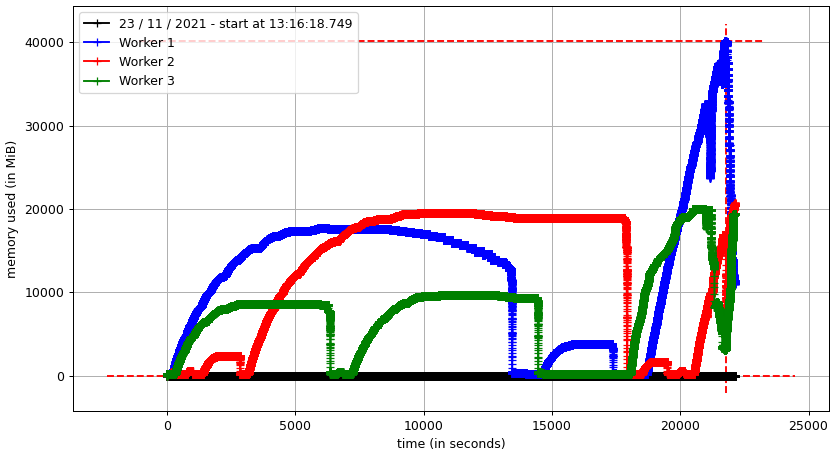
\includegraphics[scale=.5]{workers}
    \caption{Process memory usage over time (until $MemoryError$)}
    \label{fig:workers}
\end{figure}

\end{document}